\section{Related Work}

\paragraph{Game AI Benchmarks.}
Traditional benchmarks rapidly saturate, but adversarial games resist this by forcing continuous adaptation. Game AI has driven major advances: superhuman board games~\citep{silver2018general}, imperfect-information poker~\citep{brown2018superhuman, brown2019superhuman}, grandmaster-level StarCraft~II~\citep{vinyals2019grandmaster}, and human-level Diplomacy combining language models with strategic reasoning~\citep{meta2022cicero}. As Figure~\ref{fig:benchmarks} shows, RL achieves superhuman performance in fully observable settings, but this margin erodes in stochastic, partially observable environments~\citep{samuel1959}, and LLM agents consistently lag specialist RL and search systems~\citep{kaggle2025gamearena}. Hanabi~\citep{bard2020hanabi} and FightLadder~\citep{li2024fightladder} advance imperfect-information and competitive evaluation; NetHack~\citep{kuttler2020nethack} and BALROG~\citep{paglieri2024balrog} benchmark long-horizon reasoning for RL and LLM agents. However, none combines adversarial reasoning with long-horizon planning at scale, and most rely on symbolic state representations rather than visual perception. Pokémon offers a unique combination: an enormous partially observed state space, a visual RPG requiring pixel-level perception, and a massive active player base generating continuous human data and an evolving competitive metagame. The gaps between AI and humans, and between specialist and generalist AI, remain wide open.


\begin{wrapfigure}{r}{0.48\textwidth}
\centering
\vspace{-4mm}
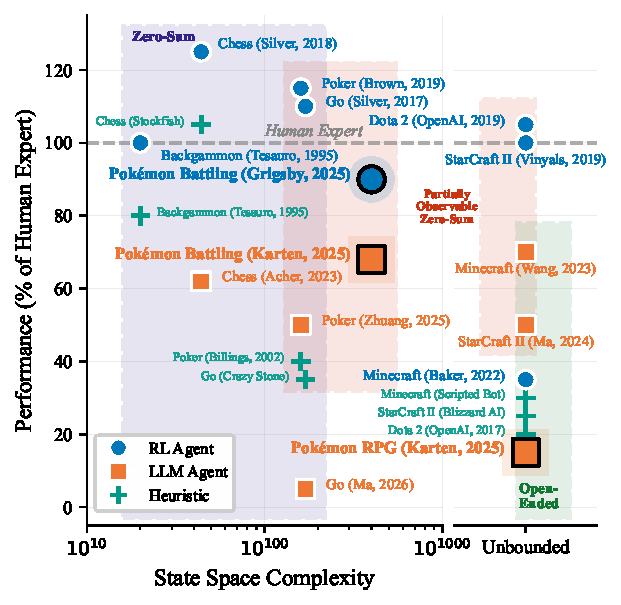
\includegraphics[width=1.05\linewidth]{figures/rl_vs_llm_benchmarks_v2.pdf}
\vspace{-6mm}
\caption{\textbf{Game Benchmarks.} Pokémon creates vast partially observable state spaces (see Appendix~\ref{sec:state-space-derivation}). Data from \cite{tesauro1995temporal, silver2018general, silver2017mastering, brown2018superhuman, brown2019superhuman, billings2002challenge, vinyals2019grandmaster, openai2019dota, baker2022video, wangvoyager, acher2024gpt4chess, ma2026mixing, yan2025pokerbench, ma2024llmstarcraft}.}
\label{fig:benchmarks}
\vspace{-6mm}
\end{wrapfigure}

\paragraph{NeurIPS Game AI Competitions.}
Standardized competitions have been important for advancing game AI. Neural MMO~\citep{liu2023neurips, suarez2023neural} benchmarks multi-agent cooperation, Lux AI~\citep{tao2024lux} targets resource management with shifting dynamics, MineRL~\citep{guss2019minerl, milani2023solvingfuzzytaskshuman, shah2022retrospective} addresses long-horizon planning in open worlds. While each advances a specific research axis, none combines adversarial partial observability with long-horizon planning at the scale of a living competitive ecosystem. \pokeagent bridges this gap: its dual-track design jointly evaluates RL and LLM approaches in high-stakes competitive play (battling) and extended sequential decision-making over thousands of steps (speedrunning), providing complementary stress tests that no single existing benchmark covers.

\paragraph{Prior Work on Pokémon AI.}
Our prior work introduced PokéChamp~\citep{karten2025pok}, combining minimax search with LLMs, and Metamon~\citep{grigsby2025human}, training RL agents on millions of human and self-play battles. On the RPG side, Puffer~\citep{pleines2025pokemon} demonstrated RL-based completion of Pokémon Red, while demonstrations from Claude~\citep{engadget2025claudeplayspokemon,anthropic2025visible}, Gemini~\citep{gemini2p5report,zhang2025geminiplayspokemon, zhang2025gemini3playspokemon}, and GPT~\citep{engadget2025gptplayspokemon} showed both the strengths and limitations of frontier models. However, each effort produced individual systems rather than reusable benchmark infrastructure: none established standardized evaluation, public leaderboards, or multi-track design for fair cross-paradigm comparison. The \pokeagent Challenge extends these efforts into a unified evaluation framework.